\documentclass{article}\usepackage[]{graphicx}\usepackage[]{color}
%% maxwidth is the original width if it is less than linewidth
%% otherwise use linewidth (to make sure the graphics do not exceed the margin)
\makeatletter
\def\maxwidth{ %
  \ifdim\Gin@nat@width>\linewidth
    \linewidth
  \else
    \Gin@nat@width
  \fi
}
\makeatother

\definecolor{fgcolor}{rgb}{0.345, 0.345, 0.345}
\newcommand{\hlnum}[1]{\textcolor[rgb]{0.686,0.059,0.569}{#1}}%
\newcommand{\hlstr}[1]{\textcolor[rgb]{0.192,0.494,0.8}{#1}}%
\newcommand{\hlcom}[1]{\textcolor[rgb]{0.678,0.584,0.686}{\textit{#1}}}%
\newcommand{\hlopt}[1]{\textcolor[rgb]{0,0,0}{#1}}%
\newcommand{\hlstd}[1]{\textcolor[rgb]{0.345,0.345,0.345}{#1}}%
\newcommand{\hlkwa}[1]{\textcolor[rgb]{0.161,0.373,0.58}{\textbf{#1}}}%
\newcommand{\hlkwb}[1]{\textcolor[rgb]{0.69,0.353,0.396}{#1}}%
\newcommand{\hlkwc}[1]{\textcolor[rgb]{0.333,0.667,0.333}{#1}}%
\newcommand{\hlkwd}[1]{\textcolor[rgb]{0.737,0.353,0.396}{\textbf{#1}}}%

\usepackage{framed}
\makeatletter
\newenvironment{kframe}{%
 \def\at@end@of@kframe{}%
 \ifinner\ifhmode%
  \def\at@end@of@kframe{\end{minipage}}%
  \begin{minipage}{\columnwidth}%
 \fi\fi%
 \def\FrameCommand##1{\hskip\@totalleftmargin \hskip-\fboxsep
 \colorbox{shadecolor}{##1}\hskip-\fboxsep
     % There is no \\@totalrightmargin, so:
     \hskip-\linewidth \hskip-\@totalleftmargin \hskip\columnwidth}%
 \MakeFramed {\advance\hsize-\width
   \@totalleftmargin\z@ \linewidth\hsize
   \@setminipage}}%
 {\par\unskip\endMakeFramed%
 \at@end@of@kframe}
\makeatother

\definecolor{shadecolor}{rgb}{.97, .97, .97}
\definecolor{messagecolor}{rgb}{0, 0, 0}
\definecolor{warningcolor}{rgb}{1, 0, 1}
\definecolor{errorcolor}{rgb}{1, 0, 0}
\newenvironment{knitrout}{}{} % an empty environment to be redefined in TeX

\usepackage{alltt}
\usepackage{CJKutf8}
%\DeclareUnicodeCharacter{0020}{~}
%\setCJKmainfont{KaiTi}
\usepackage{amsfonts}
\usepackage[%dvipdfm,  %pdflatex,pdftex这里决定运行文件的方式不同
            pdfstartview=FitH,
            CJKbookmarks=true,
            bookmarksnumbered=true,
            bookmarksopen=true,
            colorlinks, %注释掉此项则交叉引用为彩色边框(将colorlinks和pdfborder同时注释掉)
            pdfborder=001,   %注释掉此项则交叉引用为彩色边框
            linkcolor=green,
            anchorcolor=green,
            citecolor=green
            ]{hyperref}  
\usepackage{amsmath}
\usepackage{graphicx}
\title{综合评价——基于标准普尔指数的应用}
\author{徐国盛 130509030005}
\IfFileExists{upquote.sty}{\usepackage{upquote}}{}
\begin{document}
\begin{CJK*}{UTF8}{gkai}
\maketitle
\tableofcontents
\section{摘要}

标准普尔指数是典型的时间序列,对时间序列的处理有许多成熟的方法。但在这里本文不采用时间序列的方法。而是通过确立一个指标进行相关的买入卖出的决策,并通过模拟选择出稳定模型,用选择出的模型进行交易,并通过相关统计量评价加以交易表现。本文旨在方法简便易懂,对应用的相关模型的参数设置尽量最简化。


\begin{knitrout}
\definecolor{shadecolor}{rgb}{0.969, 0.969, 0.969}\color{fgcolor}\begin{kframe}
\begin{verbatim}
## [1] "GSPC"
\end{verbatim}
\end{kframe}
\end{knitrout}
\section{建立决策指标}

我们假设在接下来的~$k$~天里,如果标准普尔指数的报价变动超过~$p\%A$~,我们就会进行相应的交易(买入或卖出)。因此建立一个决策指标,它能够描述标准普尔指数在接下来~$k$~天内的趋势。当报价变动为正数,我们将买入,反之,我们将卖出。由此,我们建立的这个指标为正,说明报价将有上升的趋势,反之,报价将有下降的趋势。这里,定义日平均报价为
$$\overline{P}_i = \frac{C_i+H_i+L_i}{3}$$
其中~$C_i$~是当天的收盘价,~$H_i$~是日最高价,~$L_i$~是日最低价。
定义集合~$V_i$~,这个集合中包括的~$k$~个值为当天收盘价相对于接下来~$K$~天均价的变动半分比,定义如下
$$V_i = \left\{\frac{\overline{P}_{i+j}-C_i}{C_i}\right\}_{j=1}^k$$
我们选出集合中的~$k$~个值的绝对值大于~$p\%$~的值,对其求得的和作为我们的指示变量。
如下
$$T_i = \sum_v\{v\in V_i:v>p\%\cup v<-p\%\}$$
指示变量~$T$~意味着当其值为较大的正直时,表明多个日均值超过收盘价~$p\%$~,这是一个很好的买入信号。反之,则是一个卖出信号。

现在我们知道指示变量~$T$~是接下来~$k$~天的价格变动趋势的反应。我们的任务是预测这种行为。我们假设通过观察过去的市场行为信息,我们可以预测将来的市场价格走势。进一步讲,过去的某种行为~$p$~发生后,行为~$f$~紧跟着发生,并且这种
模式频繁发生,那么将来行为~$p$~发生时,我们可以预测~$f$~将紧接着发生。因此,我们将通过~$T$~来预测的将来的行为~$f$~。接下来我们要做的是如何描述最近的价格行为~$p$~,在这里,我们将用很多特征因子描述现在的行为~$p$~,然后通过p去预测~$T$~,进而预测将来的行为~$f$~,。

我们将注重分析收盘价,以为我们的交易决定将在每天交易结束后做出。初始的特征因子集合由多个过去基于收盘价的收益率组成。即
$$R_{i-h} = \frac{C_i-C_{i-h}}{C_{i-h}}$$
其中~$C_i$~是第~$i$~天的收盘价。我们选则~$h = 1,\dots,10$~,这样初始的特征因子集合就有~$10$~个特征因子。此外,也采用了许多技术指标作为特征因子,有平均波动因子(ATR,反应序列的波动性);随机动量指数(SMI,是一个动量指标);Wells Wilder’s方向性移动指数(ADX);Aroon 指标,用于确定序列开始趋势;Bollinger Bands, 用于比较一段时期内的波动性;Chaikin 波动;Close Location Value,将
收盘价与交易区间结合起来;Arms Ease of Movement Value;MACD振子;货币流通指数(MFI);Parabolic Stop and Reverse 以及波动指示变量。

以上这些特征因子用来预测~$T$~的将来值。
$$T = f(ATR,SMI,ADX,Aroon,BB,ChaikinVol,CLV,EMV,MACD,MFI,Volat)$$
其中~$f(\bullet)$是线性函数
\section{随机森林}
在机器学习中,随机森林是一个包含多个决策树的分类器, 并且其输出的类别是由个别树输出的类别的众数而定。 

根据下列算法而建造每棵树:

1. 用 ~$N$~ 来表示训练例子的个数,~$M$~表示变量的数目。

2. 我们会被告知一个数 ~$m$~ ,被用来决定当在一个节点上做决定时,会使用到多少个变量。~$m$~应小于~$M$~。

3. 从N个训练案例中以可重复取样的方式,取样~$N$~次,形成一组训练集(即bootstrap取样)。并使用这棵树来对剩余预测其类别,并评估其误差。

4. 对于每一个节点,随机选择~$m$~个基于此点上的变量。根据这~$m$~个变量,计算其最佳的分割方式。

5. 每棵树都会完整成长而不会剪枝(Pruning)(这有可能在建完一棵正常树状分类器后会被采用)。

\section{神经网络}
神经网络对预测问题中的变量值的大小是敏感的。因此,在用神经网络处理数据之前,对相应的数据进行预处理是十分有效的。在这里, 我们将对数据进行标准化,使其均值为~$0$~,方差为~$1$~。即用如下公式对数据进行处理。
$$y_i = \frac{x_i - \overline{x}}{\sigma_x}$$。

我们将采用向前的(feed-forward)神经网络,并且只有一层隐藏层。如下图:
\begin{figure}[ht]
\centering
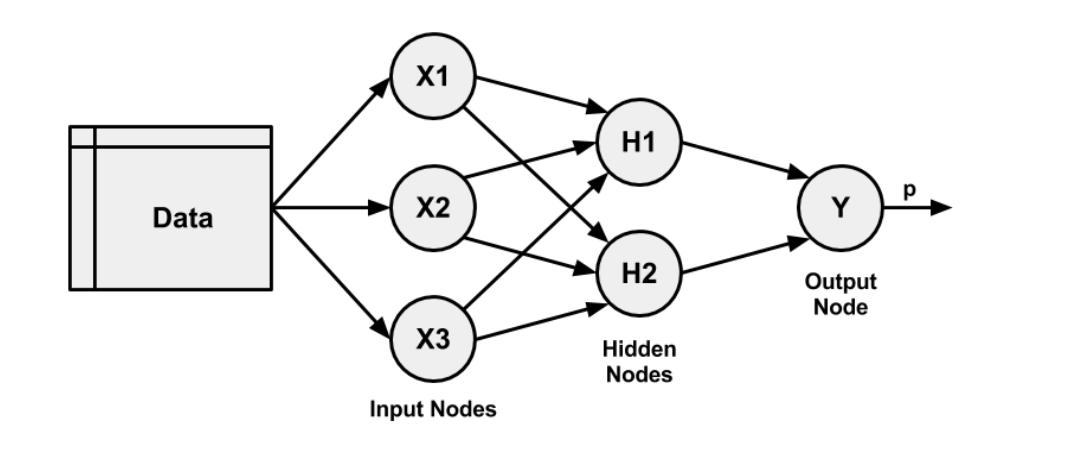
\includegraphics[width = 12cm]{./art.jpeg}
\caption{神经网络}\label{fig2.1}
\end{figure}
\section{支持向量机}
支持向量机可以用于解决回归和分类问题。由于支持向量机有很强的理论基础,因此被广泛应用。


向量机的基本思想是将原有数据映射到一个新的高唯空间,在这个高位空间里可以应用一个线性模型得到一个超平面用于分离数据,比如数据的分类问题。运用核函数将原来数据映射到高维空间。SVM是个基于核函数的线性分类器。

如果向量机将数据分为两类,那么通过最大化属于不同类别个体的分离边界,基于可以得到一个用于分类的超平面。有一种软边界的方法(soft method)允许对某些个体判断错误,当然,这需要一个量来限制,这就是损失(cost)。如下图
\begin{figure}[ht]
\centering
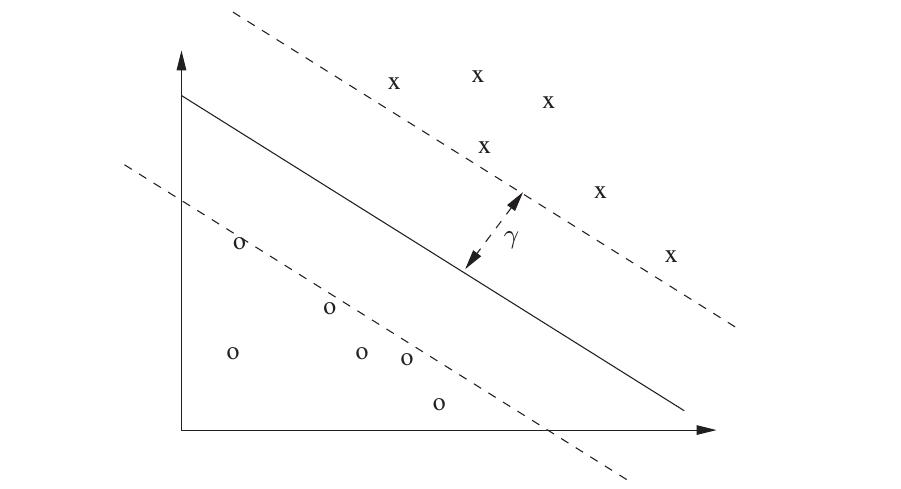
\includegraphics[width = 12cm]{./svm.jpeg}
\caption{支持向量机}
\end{figure}

对于向量机回归问题,过程与向量机分类问题是类似的。主要的不同在于误差的形式和损失的计算。这依赖于~$\epsilon-insenstive$~损失函数~$|\xi|_\epsilon$。如下:
\begin{equation*}
|\xi|_\epsilon = \left\{\begin{array}{ll}
0 & \text{if} |\xi| \leq \epsilon\\
|\xi|-\epsilon &\text{otherwise}
\end{array}\right.
\end{equation*}
\section{多元自适应样条法(Multivariate Adaptive Regression Splines)}

MARS 一般模型的形式如下:
$$mars(\mathbf{x}) = c_0 + \sum_{i=1}^kc_iB_i(\mathbf{x})$$
其中 ~$c_i$~ 是常数, ~$B_i$是基函数。
最常用的函数是 \textit{hinge} 函数,有如下形式:
$$H[-(x_i - t)] = max(0, t - x_i) \quad H[+(x_i - t)] = max(0, x_i - t)$$
其中 ~$x_i$~是写变量,  ~$t$~是一个阈值.下图为此函数一个例子的函数图像:
\begin{figure}[ht]
\centering
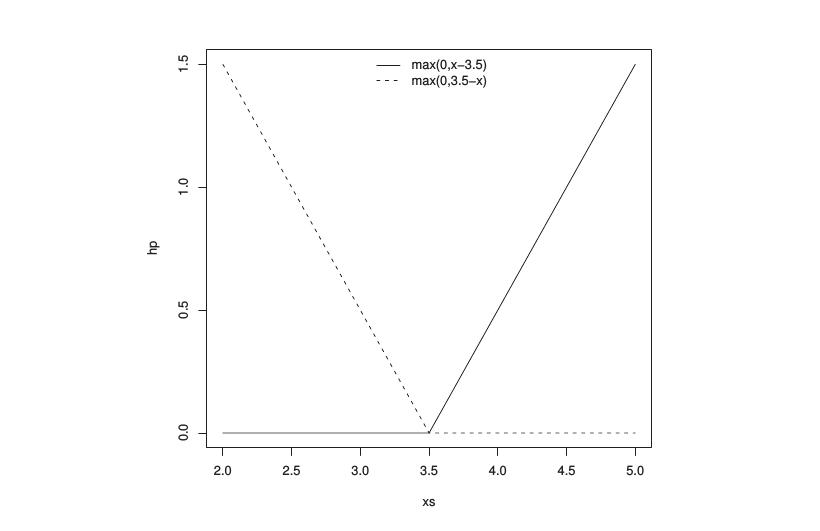
\includegraphics[width = 12cm]{./mar.jpeg}
\caption{hing函数的例子}\label{fig4.1}
\end{figure}
\section{蒙特卡罗模拟}
我们将针对相应的模型在交易区间进行蒙特卡罗模拟,我们用三种方法针对训练模型:

\textbullet 针对测试集采用单一模型

\textbullet 采用一个增长的训练集,对日期采取一个增长窗口,每当预测~$w$~天就在训练集增加~$w$~天的数据,重新训练模型,进行预测。

\textbullet 采用一个移动的训练集合,对日期采取一个移动的窗口,每当增加~$w$~天的预测,就移动窗口,移除日期最前面的陈旧的~$w$~天数据,增加~$w$~天新数据,重新训练模型,进行预测。

其三种方法可以由下图表示
\begin{figure}[ht]
\centering
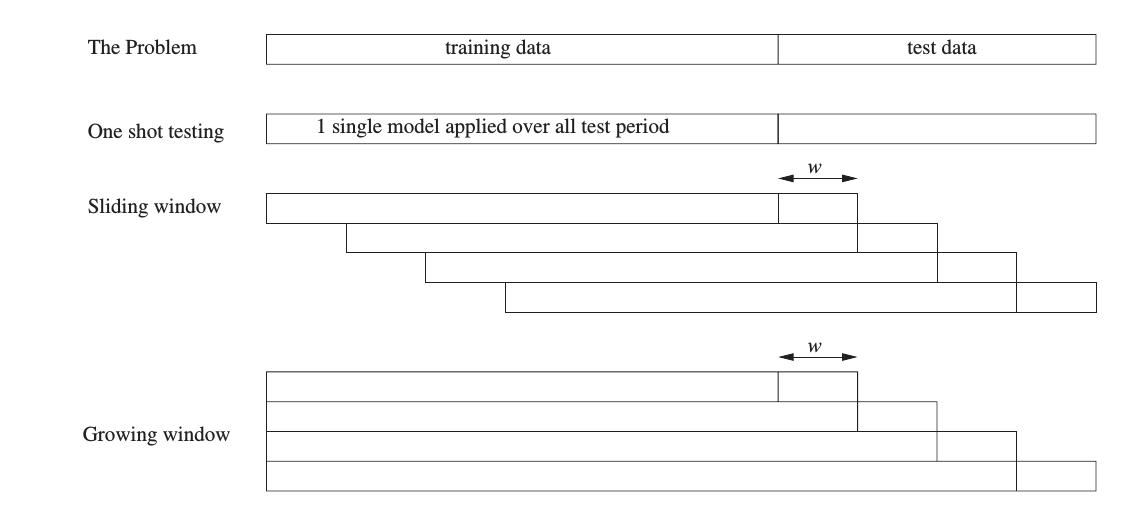
\includegraphics[width = 12cm]{./method.jpeg}
\caption{交易策略}
\end{figure}
\section{交易策略}
我们的交易系统分为多头和空头。对于长期,我们在时间~$t$~以价格~$p$~买入,并且在之后的时间~$t+x$~卖出。如果股价在将来一段时间会上升,那么就是有意义的,有盈利的可能。对于空头,将在时间~$t$~以价格~$p$~卖出,并且在将来买入。因此,我们可以认为,当价格预期上涨是,执行多头;预期下降是,进行空头。

我们将执行以下交易策略。

对于空头交易。我们将在每天交易时间结束是作出相关买入卖出决定,因为我们知道了当天的交易价格。比如在第~$t$~天,模型显示价格将下跌,也就是说,我们计算得到的~$T$~值较低,这是一个卖出信号。如果已经有了一个合同,那么模型提供的卖出信号将被忽略。如果没有合同,我们将进行一个空头交易,进行卖出。卖出命令在将来以价格~$pr$~成交。接下来,我们将进行两种操作。

\textbullet 获益买入限定。当价格为~$pr-p\%$~时,进行买入。~$p\%$~是目标利润。这一操作只有在价格达到目标价格才会执行。这一命令确定了对于刚才的空头交易,我们的目标利率。我们有10天来确定是否达到利率标准。如果在10天之后仍旧没有达到目标利率,那么,我们加以第10天的收盘价买入结束空头。

\textbullet 定损买入限定。如果价格不降反升,当价格达到~$pr+l\%$~,我们将进行买入,最终将我们的损失限制在~$l\%$~。

对于多头交易.如过模型显示价格会在寄来一段时间上升,我们将来时间~$t$~以价格~$p$~买入股票。接下来,我们将执行以下两种操作。

\textbullet 获益卖出限定。在接下来的10天里,如果价格达到或超过~$pr+p\%$~,将执行卖出操作。否则将以第10天的收盘价卖出。

\textbullet 定损卖出限定。如果在接下来的10天,价格不升反降。当价格价格降低到~$pr-l\%$~时,将被执行卖出操作
\section{实例分析}
我们这里使用的是~$1990-01-01$~到~$2009-09-15$~的标准普耳指数作为分析数据。数据来是yhaoo网站,通过网络抓取获得。
\subsection{绘制波动图,构造指标变量~$T.ind$~}
我们绘制标准普耳指数的波动图标,同时,将我们构造的指标变量绘制到图中,位于图像下部,可以但到当~$T.ind$~较大时,未来价格会有上升趋势。反之,会有下降趋势。


\begin{knitrout}
\definecolor{shadecolor}{rgb}{0.969, 0.969, 0.969}\color{fgcolor}

{\centering \includegraphics[width=\maxwidth]{figure/practice1} 

}




{\centering \includegraphics[width=\maxwidth]{figure/practice2} 

}




{\centering \includegraphics[width=\maxwidth]{figure/practice3} 

}



\end{knitrout}

\subsection{通过随机森林选出影响显著的特征因子}



我们通过逐个去除变量,通过其导致的误差大小来表示其重要性。去除变量因子后,误差越大,重要性也就越高。
\begin{knitrout}
\definecolor{shadecolor}{rgb}{0.969, 0.969, 0.969}\color{fgcolor}

{\centering \includegraphics[width=\maxwidth]{figure/check_improtance} 

}



\end{knitrout}

我们将选取重要性大于10的因子。
\begin{knitrout}
\definecolor{shadecolor}{rgb}{0.969, 0.969, 0.969}\color{fgcolor}\begin{kframe}
\begin{verbatim}
## [1] "Delt.Cl.GSPC.k.1.10.Delt.1.arithmetic"
## [2] "myATR.GSPC"                           
## [3] "myADX.GSPC"                           
## [4] "myAroon.GSPC"                         
## [5] "myCLV.GSPC"                           
## [6] "myEMV.GSPC"                           
## [7] "myVolat.GSPC"                         
## [8] "myMACD.GSPC"
\end{verbatim}
\end{kframe}
\end{knitrout}
因此,我们得到的~$T.ind$~模型为
\begin{knitrout}
\definecolor{shadecolor}{rgb}{0.969, 0.969, 0.969}\color{fgcolor}\begin{kframe}
\begin{alltt}
\hlstd{data.model} \hlkwb{<-} \hlkwd{specifyModel}\hlstd{(}\hlkwd{T.ind}\hlstd{(GSPC)} \hlopt{~} \hlkwd{Delt}\hlstd{(}\hlkwd{Cl}\hlstd{(GSPC),} \hlkwc{k} \hlstd{=} \hlnum{1}\hlstd{)} \hlopt{+}
                             \hlkwd{myATR}\hlstd{(GSPC)} \hlopt{+} \hlkwd{myADX}\hlstd{(GSPC)} \hlopt{+} \hlkwd{myEMV}\hlstd{(GSPC)}
                           \hlopt{+} \hlkwd{myVolat}\hlstd{(GSPC)} \hlopt{+} \hlkwd{myMACD}\hlstd{(GSPC)} \hlopt{+} \hlkwd{mySAR}\hlstd{(GSPC)}
                           \hlopt{+} \hlkwd{runMean}\hlstd{(}\hlkwd{Cl}\hlstd{(GSPC)))}
\end{alltt}
\end{kframe}
\end{knitrout}



在这里,我们规定~$1970$~到~$1999$~年的数据作为训练集合,以后的数据用于最终测试

\subsection{训练模型,进行预测}
\subsubsection{神经网络的测试结果}
回归测试结果
\begin{knitrout}
\definecolor{shadecolor}{rgb}{0.969, 0.969, 0.969}\color{fgcolor}\begin{kframe}
\begin{verbatim}
##     precision recall
## s      0.3735 0.3368
## b      0.2157 0.2418
## s+b    0.3287 0.3138
\end{verbatim}
\end{kframe}
\end{knitrout}

分类测试结果
\begin{knitrout}
\definecolor{shadecolor}{rgb}{0.969, 0.969, 0.969}\color{fgcolor}\begin{kframe}
\begin{verbatim}
##     precision recall
## s      0.2883 0.2246
## b      0.1825 0.2527
## s+b    0.2471 0.2287
\end{verbatim}
\end{kframe}
\end{knitrout}
\subsection{支持向量机的测试结果}
回归测试结果
\begin{knitrout}
\definecolor{shadecolor}{rgb}{0.969, 0.969, 0.969}\color{fgcolor}\begin{kframe}
\begin{verbatim}
##     precision recall
## s      0.5102 0.1754
## b         NaN 0.0000
## s+b    0.5102 0.1330
\end{verbatim}
\end{kframe}
\end{knitrout}

分类测试结果
\begin{knitrout}
\definecolor{shadecolor}{rgb}{0.969, 0.969, 0.969}\color{fgcolor}\begin{kframe}
\begin{verbatim}
## Using automatic sigma estimation (sigest) for RBF or laplace kernel
##     precision recall
## s      0.3523 0.3474
## b      0.3409 0.1648
## s+b    0.3508 0.3032
\end{verbatim}
\end{kframe}
\end{knitrout}
\subsection{多元自适应样条测试结果}
多元自适应样条只是用于回归预测分析
\begin{knitrout}
\definecolor{shadecolor}{rgb}{0.969, 0.969, 0.969}\color{fgcolor}\begin{kframe}
\begin{verbatim}
##     precision recall
## s      0.3849 0.3228
## b      0.4483 0.1429
## s+b    0.3918 0.2793
\end{verbatim}
\end{kframe}
\end{knitrout}
\subsection{构建策略函数}
见代码



\begin{knitrout}
\definecolor{shadecolor}{rgb}{0.969, 0.969, 0.969}\color{fgcolor}\begin{kframe}
\begin{verbatim}
## Money 
##  2960
## 
## Object of class tradeRecord with slots:
## 
## 	 trading: <xts object with a numeric  500 x 5  matrix>
## 	 positions: <numeric  32 x 7  matrix>
## 	 init.cap :  1e+06 
## 	 trans.cost :  5 
## 	 policy.func :  policy.1 
## 	 policy.pars : <list with  3  elements>
## 
## == Summary of a Trading Simulation with  500  days ==
## 
## Trading policy function :  policy.1 
## Policy function parameters:
## 	 exp.prof  =  0.05 
## 	 bet  =  0.2 
## 	 hold.time  =  30 
## 
## Transaction costs :  5 
## Initial Equity    :  1e+06 
## Final Equity      :  978118   Return :  -2.19 %
## Number of trading positions:  32 
## 
## Use function "tradingEvaluation()" for further stats on this simulation.
\end{verbatim}
\end{kframe}
\end{knitrout}

\begin{knitrout}
\definecolor{shadecolor}{rgb}{0.969, 0.969, 0.969}\color{fgcolor}\begin{kframe}
\begin{verbatim}
##     NTrades       NProf    PercProf          PL         Ret   RetOverBH 
##       32.00       15.00       46.88   -21882.15       -2.19      -14.20 
##       MaxDD SharpeRatio     AvgProf     AvgLoss       AvgPL     MaxProf 
##    86836.76       -0.02        5.24       -4.76       -0.07        5.26 
##     MaxLoss 
##       -4.77
\end{verbatim}
\end{kframe}
\end{knitrout}

我们可以得到根据我们的策略和相应的交易结果。
\begin{knitrout}
\definecolor{shadecolor}{rgb}{0.969, 0.969, 0.969}\color{fgcolor}

{\centering \includegraphics[width=\maxwidth]{figure/plot_tradeRecord_class} 

}


\begin{kframe}\begin{verbatim}
## Rentability =  -2.188 %
\end{verbatim}
\end{kframe}
\end{knitrout}
\begin{knitrout}
\definecolor{shadecolor}{rgb}{0.969, 0.969, 0.969}\color{fgcolor}\begin{kframe}
\begin{verbatim}
## Borrowing money ( 185420 ) for closing a short position (PosID= 90 )
## 
## == Summary of a Trading Simulation with  500  days ==
## 
## Trading policy function :  policy.2 
## Policy function parameters:
## 	 exp.prof  =  0.05 
## 	 bet  =  0.3 
## 
## Transaction costs :  5 
## Initial Equity    :  1e+06 
## Final Equity      :  1065530   Return :  6.55 %
## Number of trading positions:  117 
## 
## Use function "tradingEvaluation()" for further stats on this simulation.
\end{verbatim}
\end{kframe}
\end{knitrout}

可以发现,结果有好有坏。收益率有时为正,有时为负。
\subsection{训练集的不同位置进行模拟}
在预测过程中,当我们预测明天的指标变量,那么今天的交易信息就是已知的。我们将运用蒙特卡罗模拟得到稳定的估计。对训练集中的选定的时间~$r$~,用其气前10年的数据训练模型,后5年的数据去测试模型。我们将用蒙特卡罗模拟随机的得到时间点~$r$~,当然,~$r$~的选取是有条件限制的。如下图:
\begin{figure}[ht]
\centering
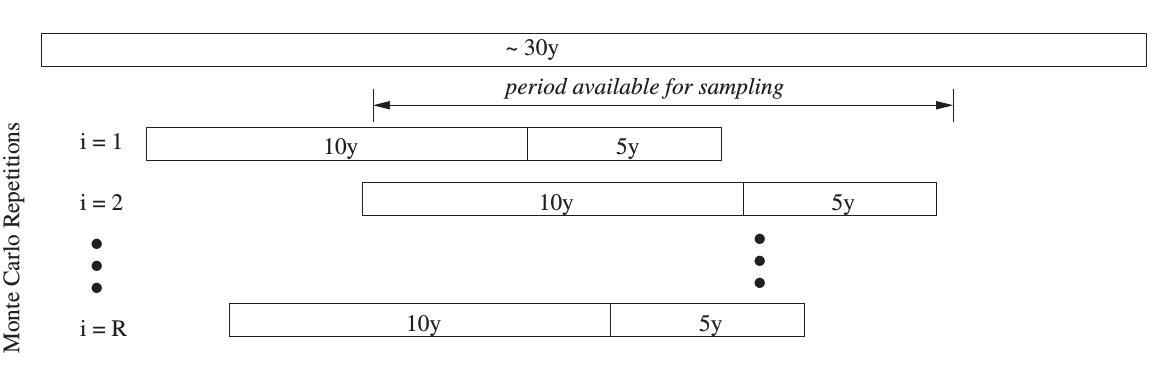
\includegraphics[width = 12cm, height = 5cm]{./moto.jpeg}
\caption{蒙特卡罗模拟的实验过程}
\end{figure}
\begin{knitrout}
\definecolor{shadecolor}{rgb}{0.969, 0.969, 0.969}\color{fgcolor}\begin{kframe}
\begin{verbatim}
## 
## == Summary of a Trading Simulation with  500  days ==
## 
## Trading policy function :  policy.2 
## Policy function parameters:
## 	 exp.prof  =  0.05 
## 	 bet  =  0.3 
## 
## Transaction costs :  5 
## Initial Equity    :  1e+06 
## Final Equity      :  163277   Return :  -83.67 %
## Number of trading positions:  254 
## 
## Use function "tradingEvaluation()" for further stats on this simulation.
\end{verbatim}
\end{kframe}

{\centering \includegraphics[width=\maxwidth]{figure/another_police_2} 

}


\begin{kframe}\begin{verbatim}
## Rentability =  -83.67 %
\end{verbatim}
\end{kframe}
\end{knitrout}





我们通过对备选模型集合进行训练,选出稳定行最好的模型。主要通过以下指标进行选择

\textbullet 收益率

\textbullet 产生收益的交易占总交易数量百分比

\textbullet 交易判断准确性

\textbullet 最大损失

\textbullet 风险系数

\begin{knitrout}
\definecolor{shadecolor}{rgb}{0.969, 0.969, 0.969}\color{fgcolor}\begin{kframe}
\begin{verbatim}
## $SP500
## $SP500$prec.sb
##           system score
## 1  slide.svmC.v5     1
## 2  slide.svmC.v6     1
## 3 slide.svmC.v13     1
## 4 slide.svmC.v14     1
## 5 slide.svmC.v21     1
## 
## $SP500$Ret
##             system   score
## 1 single.nnetR.v12 97.4240
## 2  single.svmR.v11  3.4960
## 3  slide.nnetR.v15  2.6230
## 4  single.svmC.v12  0.7875
## 5   single.svmR.v8  0.6115
## 
## $SP500$PercProf
##          system score
## 1 grow.nnetR.v5 60.42
## 2 grow.nnetR.v6 60.36
## 3 slide.svmR.v3 60.36
## 4  grow.svmR.v3 59.87
## 5 grow.nnetC.v1 59.86
## 
## $SP500$MaxDD
##           system score
## 1  slide.svmC.v5 197.4
## 2  slide.svmC.v6 197.4
## 3   grow.svmC.v5 197.4
## 4   grow.svmC.v6 197.4
## 5 slide.svmC.v13 399.3
## 
## $SP500$SharpeRatio
##           system score
## 1  slide.svmC.v5  0.02
## 2  slide.svmC.v6  0.02
## 3 slide.svmC.v13  0.02
## 4 slide.svmC.v14  0.02
## 5 slide.svmC.v21  0.02
\end{verbatim}
\end{kframe}
\end{knitrout}

我们发现交易判断准确性为~$100\%$~,这一般是不可能的,我们发现,这是由于只产生了一笔交易。
\begin{knitrout}
\definecolor{shadecolor}{rgb}{0.969, 0.969, 0.969}\color{fgcolor}\begin{kframe}
\begin{verbatim}
## 
## == Summary of a  Monte Carlo  Experiment ==
## 
##  20  repetitions Monte Carlo Simulation using: 
## 	 seed =  1234 
## 	 train size =  2540  cases 
## 	 test size =  1270  cases 
## 
## * Data sets ::  SP500
## * Learners  ::  slide.svmC.v5, slide.svmC.v6
## 
## * Summary of Experiment Results:
## 
## 
## -> Datataset:  SP500 
## 
## 	*Learner: slide.svmC.v5 
##            Ret RetOverBH PercProf NTrades
## avg     0.0250    -77.10     5.00  0.0500
## std     0.1118     33.12    22.36  0.2236
## min     0.0000   -128.01     0.00  0.0000
## max     0.5000    -33.77   100.00  1.0000
## invalid 0.0000      0.00     0.00  0.0000
## 
## 	*Learner: slide.svmC.v6 
##            Ret RetOverBH PercProf NTrades
## avg     0.0250    -77.10     5.00  0.0500
## std     0.1118     33.12    22.36  0.2236
## min     0.0000   -128.01     0.00  0.0000
## max     0.5000    -33.77   100.00  1.0000
## invalid 0.0000      0.00     0.00  0.0000
\end{verbatim}
\end{kframe}
\end{knitrout}
我们进一步增加限制条件,选出稳定模型并进行比较分析。
\begin{knitrout}
\definecolor{shadecolor}{rgb}{0.969, 0.969, 0.969}\color{fgcolor}\begin{kframe}
\begin{verbatim}
## 
## == Summary of a  Monte Carlo  Experiment ==
## 
##  20  repetitions Monte Carlo Simulation using: 
## 	 seed =  1234 
## 	 train size =  2540  cases 
## 	 test size =  1270  cases 
## 
## * Data sets ::  SP500
## * Learners  ::  single.nnetR.v12, slide.nnetR.v15, grow.nnetR.v12
## 
## * Summary of Experiment Results:
## 
## 
## -> Datataset:  SP500 
## 
## 	*Learner: single.nnetR.v12 
##         prec.sb     Ret PercProf    MaxDD SharpeRatio
## avg     0.12893   97.42    45.89  1595761    -0.01300
## std     0.06766  650.86    14.05  2205914     0.03799
## min     0.02581 -160.42    21.50   257067    -0.08000
## max     0.28696 2849.85    73.08 10142085     0.04000
## invalid 0.00000    0.00     0.00        0     0.00000
## 
## 	*Learner: slide.nnetR.v15 
##         prec.sb    Ret PercProf MaxDD SharpeRatio
## avg     0.14028  2.623   54.361 46786     0.01500
## std     0.05111  4.932    8.339 23526     0.03052
## min     0.03030 -7.030   38.890 18454    -0.04000
## max     0.22047  9.850   68.970 99458     0.05000
## invalid 0.00000  0.000    0.000     0     0.00000
## 
## 	*Learner: grow.nnetR.v12 
##         prec.sb      Ret PercProf  MaxDD SharpeRatio
## avg     0.18775   0.5445    52.66  41998     0.00600
## std     0.07964   4.3342    11.61  28252     0.03409
## min     0.04412 -10.7600    22.22  18144    -0.09000
## max     0.33077   5.3300    72.73 121886     0.05000
## invalid 0.00000   0.0000     0.00      0     0.00000
\end{verbatim}
\end{kframe}
\end{knitrout}

\begin{knitrout}
\definecolor{shadecolor}{rgb}{0.969, 0.969, 0.969}\color{fgcolor}\begin{kframe}
\begin{verbatim}
## 
## == Statistical Significance Analysis of Comparison Results ==
## 
## Baseline Learner::	 single.nnetR.v12  (Learn.1)
## 
## ** Evaluation Metric::	 prec.sb 
## 
## - Dataset: SP500 
##     Learn.1 Learn.2 sig.2 Learn.3 sig.3
## AVG 0.12893 0.14028       0.18775    + 
## STD 0.06766 0.05111       0.07964      
## 
## ** Evaluation Metric::	 Ret 
## 
## - Dataset: SP500 
##     Learn.1 Learn.2 sig.2 Learn.3 sig.3
## AVG   97.42   2.623    -   0.5445    - 
## STD  650.86   4.932        4.3342      
## 
## ** Evaluation Metric::	 PercProf 
## 
## - Dataset: SP500 
##     Learn.1 Learn.2 sig.2 Learn.3 sig.3
## AVG   45.89  54.361    +    52.66      
## STD   14.05   8.339         11.61      
## 
## ** Evaluation Metric::	 MaxDD 
## 
## - Dataset: SP500 
##     Learn.1 Learn.2 sig.2 Learn.3 sig.3
## AVG 1595761   46786    --   41998    --
## STD 2205914   23526         28252      
## 
## ** Evaluation Metric::	 SharpeRatio 
## 
## - Dataset: SP500 
##      Learn.1 Learn.2 sig.2 Learn.3 sig.3
## AVG -0.01300 0.01500    +  0.00600      
## STD  0.03799 0.03052       0.03409      
## 
## Legends:
## Learners -> Learn.1 = single.nnetR.v12 ; Learn.2 = slide.nnetR.v15 ; Learn.3 = grow.nnetR.v12 ; 
## Signif. Codes -> 0 '++' or '--' 0.001 '+' or '-' 0.05 ' ' 1
\end{verbatim}
\end{kframe}
\end{knitrout}

对每一个模型,我们都进行了20次模拟。因此,我们对选出的模型的收益率,收益率交易比重,最大损失绘制箱形图。

\begin{knitrout}
\definecolor{shadecolor}{rgb}{0.969, 0.969, 0.969}\color{fgcolor}

{\centering \includegraphics[width=\maxwidth]{figure/comExp_plot} 

}



\end{knitrout}
\begin{knitrout}
\definecolor{shadecolor}{rgb}{0.969, 0.969, 0.969}\color{fgcolor}\begin{kframe}
\begin{verbatim}
## 
## Learner::  "single" 
## 
## Parameter values
## 	 learner  =  "nnetR" 
## 	 linout  =  TRUE 
## 	 trace  =  FALSE 
## 	 maxit  =  750 
## 	 size  =  10 
## 	 decay  =  0.01 
## 	 policy.func  =  "pol3"
\end{verbatim}
\end{kframe}
\end{knitrout}
最终,我们用最后9年的数据进行测试
\begin{knitrout}
\definecolor{shadecolor}{rgb}{0.969, 0.969, 0.969}\color{fgcolor}\begin{kframe}
\begin{verbatim}
## *****************************************
## *********************
##                   Ret RetOverBH MaxDD SharpeRatio NTrades PercProf
## slide.nnetR.v15  0.00      0.38     0         NaN       0        0
## grow.nnetR.v12  -0.72     -0.34  8325       -0.36       1        0
\end{verbatim}
\end{kframe}
\end{knitrout}

最终,我们列出最好的模型的性质记过
\begin{knitrout}
\definecolor{shadecolor}{rgb}{0.969, 0.969, 0.969}\color{fgcolor}\begin{kframe}
\begin{verbatim}
## 
## Learner::  "slide" 
## 
## Parameter values
## 	 learner  =  "nnetR" 
## 	 relearn.step  =  60 
## 	 linout  =  TRUE 
## 	 trace  =  FALSE 
## 	 maxit  =  750 
## 	 size  =  10 
## 	 decay  =  0.01 
## 	 policy.func  =  "pol2"
\end{verbatim}
\end{kframe}
\end{knitrout}

通过绘制交易图,观察模型表现

\begin{knitrout}
\definecolor{shadecolor}{rgb}{0.969, 0.969, 0.969}\color{fgcolor}

{\centering \includegraphics[width=\maxwidth]{figure/plot_trade_res} 

}


\begin{kframe}\begin{verbatim}
## Rentability =  11.05 %
\end{verbatim}
\end{kframe}
\end{knitrout}

进一步得到相应的收益率,包括月收益率
\begin{knitrout}
\definecolor{shadecolor}{rgb}{0.969, 0.969, 0.969}\color{fgcolor}

{\centering \includegraphics[width=\maxwidth]{figure/PerformanceAnalytics1} 

}


\begin{kframe}\begin{verbatim}
##            yearly.returns
## 2000-12-29      0.0559194
## 2001-12-31      0.0700963
## 2002-12-31      0.0354678
## 2003-12-31     -0.0220358
## 2004-12-31      0.0094184
## 2005-12-30      0.0003918
\end{verbatim}
\end{kframe}

{\centering \includegraphics[width=\maxwidth]{figure/PerformanceAnalytics2} 

}



\end{knitrout}
\begin{knitrout}
\definecolor{shadecolor}{rgb}{0.969, 0.969, 0.969}\color{fgcolor}\begin{kframe}
\begin{verbatim}
##       1月  2月  3月  4月  5月  6月  7月  8月  9月 10月 11月 12月    x
## 2000  0.0  0.3  0.0  0.2  0.0 -0.2  0.2  0.2  0.0  0.0  0.0  0.1  0.7
## 2001 -0.1 -0.3  0.2 -0.1 -0.1  0.0 -0.1 -0.1  0.4  0.0  0.0  0.0 -0.1
## 2002  0.0  0.1  0.0 -0.2  0.0  0.0  0.2  0.0 -0.6 -0.1  0.0  0.0 -0.8
## 2003 -0.3 -0.1  0.4  0.0  0.0  0.0  0.0  0.0  0.0  0.0  0.0  0.0  0.0
## 2004  0.0  0.0  0.0  0.1  0.0 -0.1  0.0  0.0  0.0  0.0  0.0  0.0  0.1
## 2005  0.0  0.0  0.0 -0.2  0.0  0.0  0.0  0.0  0.0  0.0  0.0  0.0 -0.2
## 2006  0.0  0.0  0.0  0.0  0.0  0.0  0.0  0.0  0.0  0.0  0.0  0.0   NA
## 2007  0.0  0.0  0.0  0.0  0.0  0.0  0.2 -0.2  0.0  0.0 -0.2  0.1  0.0
## 2008 -0.3  0.5  0.0  0.1  0.0  0.0  0.3  0.3  0.9  0.3  0.2  0.3  2.4
## 2009 -0.5 -0.5 -0.2  0.0  0.0  0.0  0.0  0.0   NA   NA   NA   NA -1.1
\end{verbatim}
\end{kframe}
\end{knitrout}
\begin{knitrout}
\definecolor{shadecolor}{rgb}{0.969, 0.969, 0.969}\color{fgcolor}\begin{kframe}
\begin{verbatim}
##                                     x
## Semi Deviation                 0.0015
## Gain Deviation                 0.0021
## Loss Deviation                 0.0022
## Downside Deviation (MAR=210%)  0.0086
## Downside Deviation (Rf=0%)     0.0015
## Downside Deviation (0%)        0.0015
## Maximum Drawdown               0.0803
## Historical VaR (95%)          -0.0036
## Historical ES (95%)           -0.0057
## Modified VaR (95%)            -0.0033
## Modified ES (95%)             -0.0053
\end{verbatim}
\end{kframe}
\end{knitrout}
\section{几点重要的说明}

\textbullet 本文不是论文,尽管也尽量写成了论文的格式。在文中没有标注引用。

\textbullet 本文中所涉及的程序代码较长,尽管文章也附上了程序,当不建议读者阅读纸质代码,在\url{http://rpubs.com/appsoner/zonghepingjia}中,提供了本文中相关的所有的代码,并且配有相应的运算结果。如果想运行相关代码,强烈建议在网页上复制代码然后粘贴运行。

\textbullet 本文模拟基于ubuntu系统13.04 LTS, 酷睿双核,主频2.34GHZ,4G内存

\textbullet 本文之附上部分代码。

\textbullet 模拟部分是本文的重点。
\section{附录(部分代码)}
\begin{knitrout}
\definecolor{shadecolor}{rgb}{0.969, 0.969, 0.969}\color{fgcolor}\begin{kframe}
\begin{alltt}
\hlstd{policy.1} \hlkwb{<-} \hlkwa{function}\hlstd{(}\hlkwc{signals}\hlstd{,} \hlkwc{market}\hlstd{,} \hlkwc{opened.pos}\hlstd{,} \hlkwc{money}\hlstd{,}
                     \hlkwc{bet} \hlstd{=} \hlnum{0.2}\hlstd{,} \hlkwc{hold.time} \hlstd{=} \hlnum{10}\hlstd{,}
                     \hlkwc{exp.prof} \hlstd{=} \hlnum{0.025}\hlstd{,} \hlkwc{max.loss} \hlstd{=} \hlnum{0.05}\hlstd{)}
\hlstd{\{}
  \hlstd{d} \hlkwb{<-} \hlkwd{NROW}\hlstd{(market)} \hlcom{# this is the ID of today}
  \hlstd{orders} \hlkwb{<-} \hlkwa{NULL}
  \hlstd{nOs} \hlkwb{<-} \hlkwd{NROW}\hlstd{(opened.pos)}
  \hlcom{#nothing to do!}
  \hlkwa{if}\hlstd{(}\hlopt{!}\hlstd{nOs} \hlopt{&&} \hlstd{signals[d]} \hlopt{==} \hlstr{'h'}\hlstd{)} \hlkwd{return} \hlstd{(orders)}
  \hlcom{#First lets check if we can open new positions}
  \hlcom{#i)long positions}
  \hlkwa{if}\hlstd{(signals[d]} \hlopt{==} \hlstr{'b'} \hlopt{&& !}\hlstd{nOs)\{}
    \hlstd{quant} \hlkwb{<-} \hlkwd{round}\hlstd{(bet}\hlopt{*}\hlstd{money}\hlopt{/}\hlstd{market[d,} \hlstr{'Close'}\hlstd{],} \hlnum{0}\hlstd{)}
    \hlkwd{print}\hlstd{(quant)}
    \hlkwa{if}\hlstd{(quant} \hlopt{>} \hlnum{0}\hlstd{)}
      \hlstd{orders} \hlkwb{<-} \hlkwd{rbind}\hlstd{(orders,} \hlkwd{data.frame}\hlstd{(}\hlkwc{order} \hlstd{=} \hlkwd{c}\hlstd{(}\hlnum{1}\hlstd{,} \hlopt{-}\hlnum{1}\hlstd{,} \hlopt{-}\hlnum{1}\hlstd{),}
                                         \hlkwc{order.type} \hlstd{=} \hlkwd{c}\hlstd{(}\hlnum{1}\hlstd{,} \hlnum{2}\hlstd{,} \hlnum{3}\hlstd{),}
                                         \hlkwc{val} \hlstd{=} \hlkwd{c}\hlstd{(quant,}
                                                 \hlstd{market[d,} \hlstr{'Close'}\hlstd{]}\hlopt{*}
                                                   \hlstd{(}\hlnum{1}\hlopt{+}\hlstd{exp.prof),}
                                                 \hlstd{market[d,} \hlstr{'Close'}\hlstd{]}\hlopt{*}
                                                   \hlstd{(}\hlnum{1} \hlopt{-} \hlstd{max.loss)),}
                                         \hlkwc{action} \hlstd{=} \hlkwd{c}\hlstd{(}\hlstr{'open'}\hlstd{,} \hlstr{'close'}\hlstd{,}
                                                    \hlstr{'close'}\hlstd{),}
                                         \hlkwc{posID} \hlstd{=} \hlkwd{c}\hlstd{(}\hlnum{NA}\hlstd{,} \hlnum{NA}\hlstd{,} \hlnum{NA}\hlstd{)}
                                         \hlstd{)}
                      \hlstd{)}
    \hlcom{#ii) short positions}
  \hlstd{\}} \hlkwa{else if} \hlstd{(signals[d]} \hlopt{==} \hlstr{'s'} \hlopt{&& !}\hlstd{nOs) \{}
    \hlcom{#This is the nr of stocks we already need to buy}
    \hlcom{#because of currently opened short positions}
    \hlstd{need2buy} \hlkwb{<-} \hlkwd{sum}\hlstd{(opened.pos[opened.pos[,} \hlstr{'pos.type'}\hlstd{]} \hlopt{== -}\hlnum{1}\hlstd{,}
                               \hlstr{"N.stocks"}\hlstd{])}\hlopt{*}\hlstd{market[d,} \hlstr{'Close'}\hlstd{]}
    \hlstd{quant} \hlkwb{<-} \hlkwd{round}\hlstd{(bet}\hlopt{*}\hlstd{(money}\hlopt{-}\hlstd{need2buy)}\hlopt{/}\hlstd{market[d,} \hlstr{'Close'}\hlstd{],} \hlnum{0}\hlstd{)}
    \hlkwa{if}\hlstd{(quant} \hlopt{>} \hlnum{0}\hlstd{)}
      \hlstd{orders} \hlkwb{<-} \hlkwd{rbind}\hlstd{(orders,}
                      \hlkwd{data.frame}\hlstd{(}\hlkwc{order} \hlstd{=} \hlkwd{c}\hlstd{(}\hlopt{-}\hlnum{1}\hlstd{,} \hlnum{1}\hlstd{,} \hlnum{1}\hlstd{),}
                                 \hlkwc{order.type} \hlstd{=} \hlkwd{c}\hlstd{(}\hlnum{1}\hlstd{,} \hlnum{2}\hlstd{,} \hlnum{3}\hlstd{),}
                                 \hlkwc{val} \hlstd{=} \hlkwd{c}\hlstd{(quant, market[d,} \hlstr{'Close'}\hlstd{]}
                                         \hlopt{*}\hlstd{(}\hlnum{1}\hlopt{-}\hlstd{exp.prof),}
                                         \hlstd{market[d,} \hlstr{'Close'}\hlstd{]}\hlopt{*}
                                           \hlstd{(}\hlnum{1} \hlopt{+} \hlstd{max.loss)),}
                                 \hlkwc{action} \hlstd{=} \hlkwd{c}\hlstd{(}\hlstr{'open'}\hlstd{,} \hlstr{'close'}\hlstd{,}
                                            \hlstr{'close'}\hlstd{),}
                                 \hlkwc{posID} \hlstd{=} \hlkwd{c}\hlstd{(}\hlnum{NA}\hlstd{,} \hlnum{NA}\hlstd{,} \hlnum{NA}\hlstd{)}
                                 \hlstd{)}
                      \hlstd{)}
  \hlstd{\}}
  \hlcom{#let's check if we need to close positions}
  \hlcom{#because their holding time is over }
  \hlkwa{if}\hlstd{(nOs)}
    \hlkwa{for}\hlstd{(i} \hlkwa{in} \hlnum{1}\hlopt{:}\hlstd{nOs) \{}
      \hlkwa{if}\hlstd{(d} \hlopt{-} \hlstd{opened.pos[i,} \hlstr{'Odate'}\hlstd{]} \hlopt{>=} \hlstd{hold.time)}
        \hlstd{orders} \hlkwb{<-} \hlkwd{rbind}\hlstd{(orders,}
                        \hlkwd{data.frame}\hlstd{(}\hlkwc{order} \hlstd{=} \hlopt{-}\hlstd{opened.pos[i,} \hlstr{'pos.type'}\hlstd{],}
                                   \hlkwc{order.type} \hlstd{=} \hlnum{1}\hlstd{,}
                                   \hlkwc{val} \hlstd{=} \hlnum{NA}\hlstd{,}
                                   \hlkwc{action} \hlstd{=} \hlstr{'close'}\hlstd{,}
                                   \hlkwc{posID} \hlstd{=} \hlkwd{rownames}\hlstd{(opened.pos)[i]}
                                   \hlstd{)}
                        \hlstd{)}
        \hlstd{\}}
  \hlstd{orders}
\hlstd{\}}
\end{alltt}
\end{kframe}
\end{knitrout}
\begin{knitrout}
\definecolor{shadecolor}{rgb}{0.969, 0.969, 0.969}\color{fgcolor}\begin{kframe}
\begin{alltt}
\hlstd{policy.2} \hlkwb{<-} \hlkwa{function}\hlstd{(}\hlkwc{signals}\hlstd{,} \hlkwc{market}\hlstd{,} \hlkwc{opened.pos}\hlstd{,} \hlkwc{money}\hlstd{,}
                     \hlkwc{bet} \hlstd{=} \hlnum{0.2}\hlstd{,} \hlkwc{exp.prof} \hlstd{=} \hlnum{0.025}\hlstd{,}
                     \hlkwc{max.loss} \hlstd{=} \hlnum{0.05}\hlstd{)}
\hlstd{\{}
  \hlstd{d} \hlkwb{<-} \hlkwd{NROW}\hlstd{(market)} \hlcom{#this is the ID of today}
  \hlstd{orders} \hlkwb{<-} \hlkwa{NULL}
  \hlstd{nOs} \hlkwb{<-} \hlkwd{NROW}\hlstd{(opened.pos)}
  \hlcom{#nothing to do}
  \hlkwa{if}\hlstd{(}\hlopt{!}\hlstd{nOs} \hlopt{&&} \hlstd{signals[d]} \hlopt{==} \hlstr{'h'}\hlstd{)} \hlkwd{return} \hlstd{(orders)}
  \hlcom{#First lets check if we can open new positions}
  \hlcom{# i) long positions}
  \hlkwa{if} \hlstd{(signals[d]} \hlopt{==} \hlstr{'b'}\hlstd{)\{}
    \hlstd{quant} \hlkwb{<-} \hlkwd{round}\hlstd{(bet}\hlopt{*}\hlstd{money}\hlopt{/}\hlstd{market[d,} \hlstr{'Close'}\hlstd{],} \hlnum{0}\hlstd{)}
   \hlcom{# print(quant)}
    \hlkwa{if} \hlstd{(quant} \hlopt{>} \hlnum{0}\hlstd{)}
      \hlstd{orders} \hlkwb{<-} \hlkwd{rbind}\hlstd{(orders,}
                      \hlkwd{data.frame}\hlstd{(}\hlkwc{order} \hlstd{=} \hlkwd{c}\hlstd{(}\hlnum{1}\hlstd{,} \hlopt{-}\hlnum{1}\hlstd{,} \hlopt{-}\hlnum{1}\hlstd{),}
                                 \hlkwc{order.type} \hlstd{=} \hlkwd{c}\hlstd{(}\hlnum{1}\hlstd{,} \hlnum{2}\hlstd{,} \hlnum{3}\hlstd{),}
                                 \hlkwc{val} \hlstd{=} \hlkwd{c}\hlstd{(quant,}
                                         \hlstd{market[d,} \hlstr{'Close'}\hlstd{]}\hlopt{*}
                                           \hlstd{(}\hlnum{1}\hlopt{+}\hlstd{exp.prof),}
                                         \hlstd{market[d,} \hlstr{'Close'}\hlstd{]}\hlopt{*}
                                           \hlstd{(}\hlnum{1}\hlopt{-}\hlstd{max.loss)}
                                         \hlstd{),}
                                 \hlkwc{action} \hlstd{=} \hlkwd{c}\hlstd{(}\hlstr{'open'}\hlstd{,} \hlstr{'close'}\hlstd{,}
                                            \hlstr{'close'}\hlstd{),}
                                 \hlkwc{posID} \hlstd{=} \hlkwd{c}\hlstd{(}\hlnum{NA}\hlstd{,} \hlnum{NA}\hlstd{,} \hlnum{NA}\hlstd{)}
                                 \hlstd{)}
                      \hlstd{)}
  \hlstd{\}} \hlkwa{else if} \hlstd{(signals[d]} \hlopt{==} \hlstr{'s'}\hlstd{) \{}
    \hlcom{#this is the money already commited to buy stocks}
    \hlcom{#because of currently opened short positions}
    \hlstd{need2buy} \hlkwb{<-} \hlkwd{sum}\hlstd{(opened.pos[opened.pos[,} \hlstr{'pos.type'}\hlstd{]} \hlopt{== -}\hlnum{1}\hlstd{,}
                               \hlstr{"N.stocks"}\hlstd{])}\hlopt{*}\hlstd{market[d,} \hlstr{'Close'}\hlstd{]}
    \hlstd{quant} \hlkwb{<-} \hlkwd{round}\hlstd{(bet}\hlopt{*}\hlstd{(money} \hlopt{-} \hlstd{need2buy)}\hlopt{/}\hlstd{market[d,} \hlstr{'Close'}\hlstd{],} \hlnum{0}\hlstd{)}
    \hlkwa{if}\hlstd{(quant} \hlopt{>}\hlnum{0}\hlstd{)}
      \hlstd{orders} \hlkwb{<-} \hlkwd{rbind}\hlstd{(orders,}
                      \hlkwd{data.frame}\hlstd{(}\hlkwc{order} \hlstd{=} \hlkwd{c}\hlstd{(}\hlopt{-}\hlnum{1}\hlstd{,} \hlnum{1}\hlstd{,} \hlnum{1}\hlstd{),}
                                 \hlkwc{order.type} \hlstd{=} \hlkwd{c}\hlstd{(}\hlnum{1}\hlstd{,} \hlnum{2}\hlstd{,} \hlnum{3}\hlstd{),}
                                 \hlkwc{val} \hlstd{=} \hlkwd{c}\hlstd{(quant,}
                                         \hlstd{market[d,} \hlstr{'Close'}\hlstd{]}\hlopt{*}
                                           \hlstd{(}\hlnum{1}\hlopt{-}\hlstd{exp.prof),}
                                         \hlstd{market[d,} \hlstr{'Close'}\hlstd{]}\hlopt{*}
                                           \hlstd{(}\hlnum{1} \hlopt{+} \hlstd{max.loss)}
                                         \hlstd{),}
                                 \hlkwc{action} \hlstd{=} \hlkwd{c}\hlstd{(}\hlstr{'open'}\hlstd{,} \hlstr{'close'}\hlstd{,} \hlstr{'close'}\hlstd{),}
                                 \hlkwc{posID} \hlstd{=} \hlkwd{c}\hlstd{(}\hlnum{NA}\hlstd{,} \hlnum{NA}\hlstd{,} \hlnum{NA}\hlstd{)}
                                 \hlstd{)}
                      \hlstd{)}
  \hlstd{\}}
  \hlstd{orders}
\hlstd{\}}
\end{alltt}
\end{kframe}
\end{knitrout}
\begin{knitrout}
\definecolor{shadecolor}{rgb}{0.969, 0.969, 0.969}\color{fgcolor}\begin{kframe}
\begin{alltt}
\hlstd{start} \hlkwb{<-} \hlnum{1}
\hlstd{len.tr} \hlkwb{<-} \hlnum{1000}
\hlstd{len.ts} \hlkwb{<-} \hlnum{500}
\hlstd{tr} \hlkwb{<-} \hlstd{start}\hlopt{:}\hlstd{(start}\hlopt{+}\hlstd{len.tr}\hlopt{-}\hlnum{1}\hlstd{)}
\hlstd{ts} \hlkwb{<-} \hlstd{(start} \hlopt{+} \hlstd{len.tr)}\hlopt{:}\hlstd{(start}\hlopt{+}\hlstd{len.tr}\hlopt{+}\hlstd{len.ts}\hlopt{-}\hlnum{1}\hlstd{)}
\hlcom{#generate the quotes for the testing period}
\hlkwd{data}\hlstd{(GSPC)}
\hlstd{date} \hlkwb{<-} \hlkwd{rownames}\hlstd{(Tdata.train[start}\hlopt{+}\hlstd{len.tr, ])}
\hlstd{market} \hlkwb{<-} \hlstd{GSPC[}\hlkwd{paste}\hlstd{(date,} \hlstr{'/'}\hlstd{,} \hlkwc{sep} \hlstd{=} \hlstr{''}\hlstd{)][}\hlnum{1}\hlopt{:}\hlstd{len.ts]}
\hlcom{#learining the model and obtaining its signal predictions}
\hlkwd{library}\hlstd{(e1071)}
\hlstd{s} \hlkwb{<-} \hlkwd{svm}\hlstd{(Tform, Tdata.train[tr, ],} \hlkwc{cost} \hlstd{=} \hlnum{10}\hlstd{,} \hlkwc{gamma} \hlstd{=} \hlnum{0.01}\hlstd{)}
\hlstd{p} \hlkwb{<-} \hlkwd{predict}\hlstd{(s, Tdata.train[ts, ])}
\hlstd{sig} \hlkwb{<-} \hlkwd{trading.signals}\hlstd{(p,} \hlnum{0.1}\hlstd{,} \hlopt{-}\hlnum{0.1}\hlstd{)}
\hlcom{#now using the simulated trader}
\hlstd{t1} \hlkwb{<-} \hlkwd{trading.simulator}\hlstd{(market, sig,} \hlstr{'policy.1'}\hlstd{,}
                      \hlkwd{list}\hlstd{(}\hlkwc{exp.prof} \hlstd{=} \hlnum{0.05}\hlstd{,} \hlkwc{bet} \hlstd{=} \hlnum{0.2}\hlstd{,}
                           \hlkwc{hold.time} \hlstd{=} \hlnum{30}\hlstd{))}
\hlstd{t1}
\hlkwd{summary}\hlstd{(t1)}
\end{alltt}
\end{kframe}
\end{knitrout}


\end{CJK*}
\end{document}




